% Chapter Template

\chapter{System Components} % Main chapter title

\label{Chapter2} % Change X to a consecutive number; for referencing this chapter elsewhere, use \ref{ChapterX}

\lhead{Chapter 2. \emph{System Components}} % Change X to a consecutive number; this is for the header on each page - perhaps a shortened title

%----------------------------------------------------------------------------------------
%	SECTION 1
%----------------------------------------------------------------------------------------
\section{Humanoid Robot}

NAO\cite{NaoTheRobot} is a humanoid robot developed in the year 2006 by Albebaran Robotics, the company which has proved itself in the development of interactive social robots. The intended scenarios include reception, assistance, home care, entertainment and even autism therapy. Nao has become a standard in academic world for research and education. In 2013, Aldebaran launched \emph{Autism Solution for Kids}\cite{ASKNao} initiative which offers a new teaching approach to teachers and children with autism. Clearly Nao is one of most sold (about 5000) humanoid robots worldwide. Therefore developing HRI solutions targeting Nao will definitely attract huge audience which in turn will help to receive more technical inputs and contribution for solving the problem under study.
\begin{figure}
\centering
\begin{subfigure}[b]{0.8\textwidth}
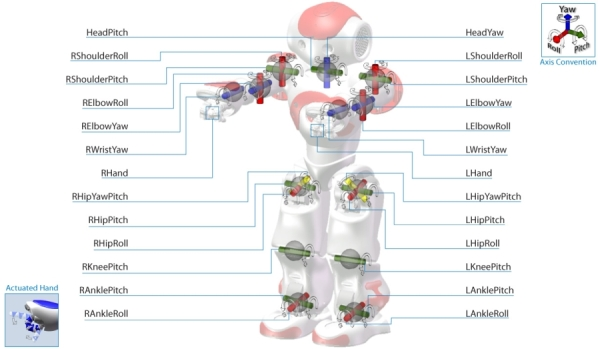
\includegraphics[width=\textwidth]{assets/nao_hardware_jointname.jpg}
\caption{Joints}
\label{fig:naojoint}
\end{subfigure}
\begin{subfigure}[b]{0.3\textwidth}
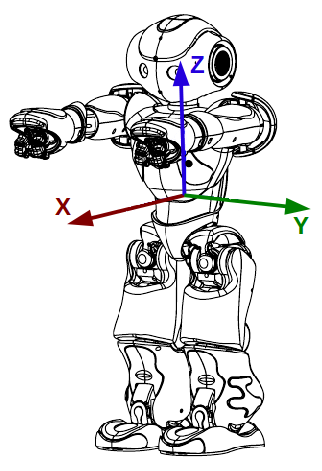
\includegraphics[width=\textwidth]{assets/hardware_inertialunit1.png}
%http://www.microsoftstore.com/store/msusa/en_US/pdp/Kinect-for-Windows/productID.253769800
\caption{Torso reference frame}
\label{fig:naoreference}
\end{subfigure}
%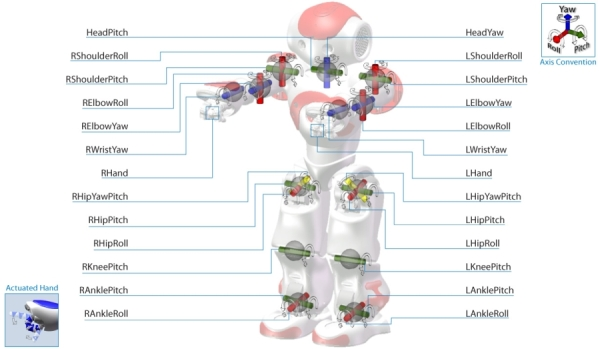
\includegraphics[width=\textwidth]{assets/nao_hardware_jointname.jpg}
%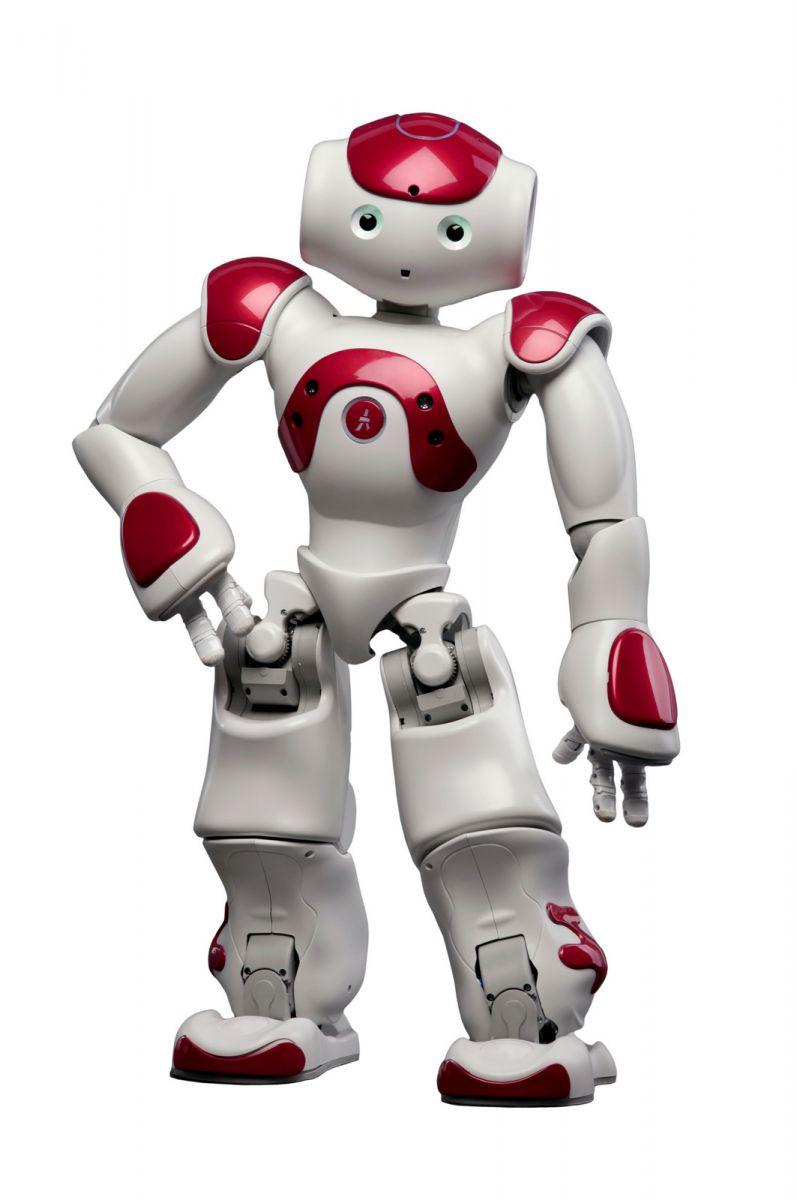
\includegraphics[width=0.2\textwidth]{assets/nao_image1.jpg}
\caption[NAO Humanoid Robot]{NAO Humanoid Robot. {Adopted from \cite{NaoTheRobot}}}
\label{fig:naorobot}
\end{figure}%

	 NAO is a programmable, 58 cm tall robot with 25 DOF whose key elements are electric motors and actuators. As far as the NAO's motion is considered, its walking uses a simple dynamic model (Linear inverted pendulum) and quadratic programming and is stabilized using the feedback from the joint sensor. NAO sees using two 1220 p cameras, which can capture up to 30 FPS. The first camera, located on NAO’s forehead, scans the horizon, while the second located at mouth level scans the immediate surroundings. NAO contains a set of algorithms for detecting and recognizing faces and shapes. It is possible to develop user-modules to interace with OpenCV library and exploit the power of the algorithms that ships with OpenCV. NAO has the ability to localize the sound source based on an approach known as “Time Difference of Arrival". The difference in the arrival of sound at each of NAO’s four microphones (Interaural time difference) is computed to determine the location of the emitting source. Besides cameras and microphones, NAO has capacitive sensors positioned on top of its head in three sections and its hands with the help of which information can be also communicated through touch. NAO is equipped with two SONAR channels for obstacle detection (range 5cm$\sim$3m). It currently supports Wi-Fi (bgn) and Ethernet and it also has infrared transceivers that allow connection to objects in the environment. It is powered with Intel atom CPU that runs a linux kernel and support Aldebaran's NAOqi middleware, a cross platform distributed environment. Aldebaran also provides Choregraphe\cite{pot2009choregraphe} which is a visual programming tool for designing behaviors and it is a specific module of NaoQi running on development computer. Choregraphe gives access in a very intuitive way to all the functions provided by NaoQi. NaoQi provides Python and URBI\cite{baillie2008urbi} interpreters. NaoQi makes it possible sequential, parallel or event-based execution of behaviors through its powerful command framework.
\section{Human motion capture}
\label{sec:motion_capture}
\begin{figure}
\centering
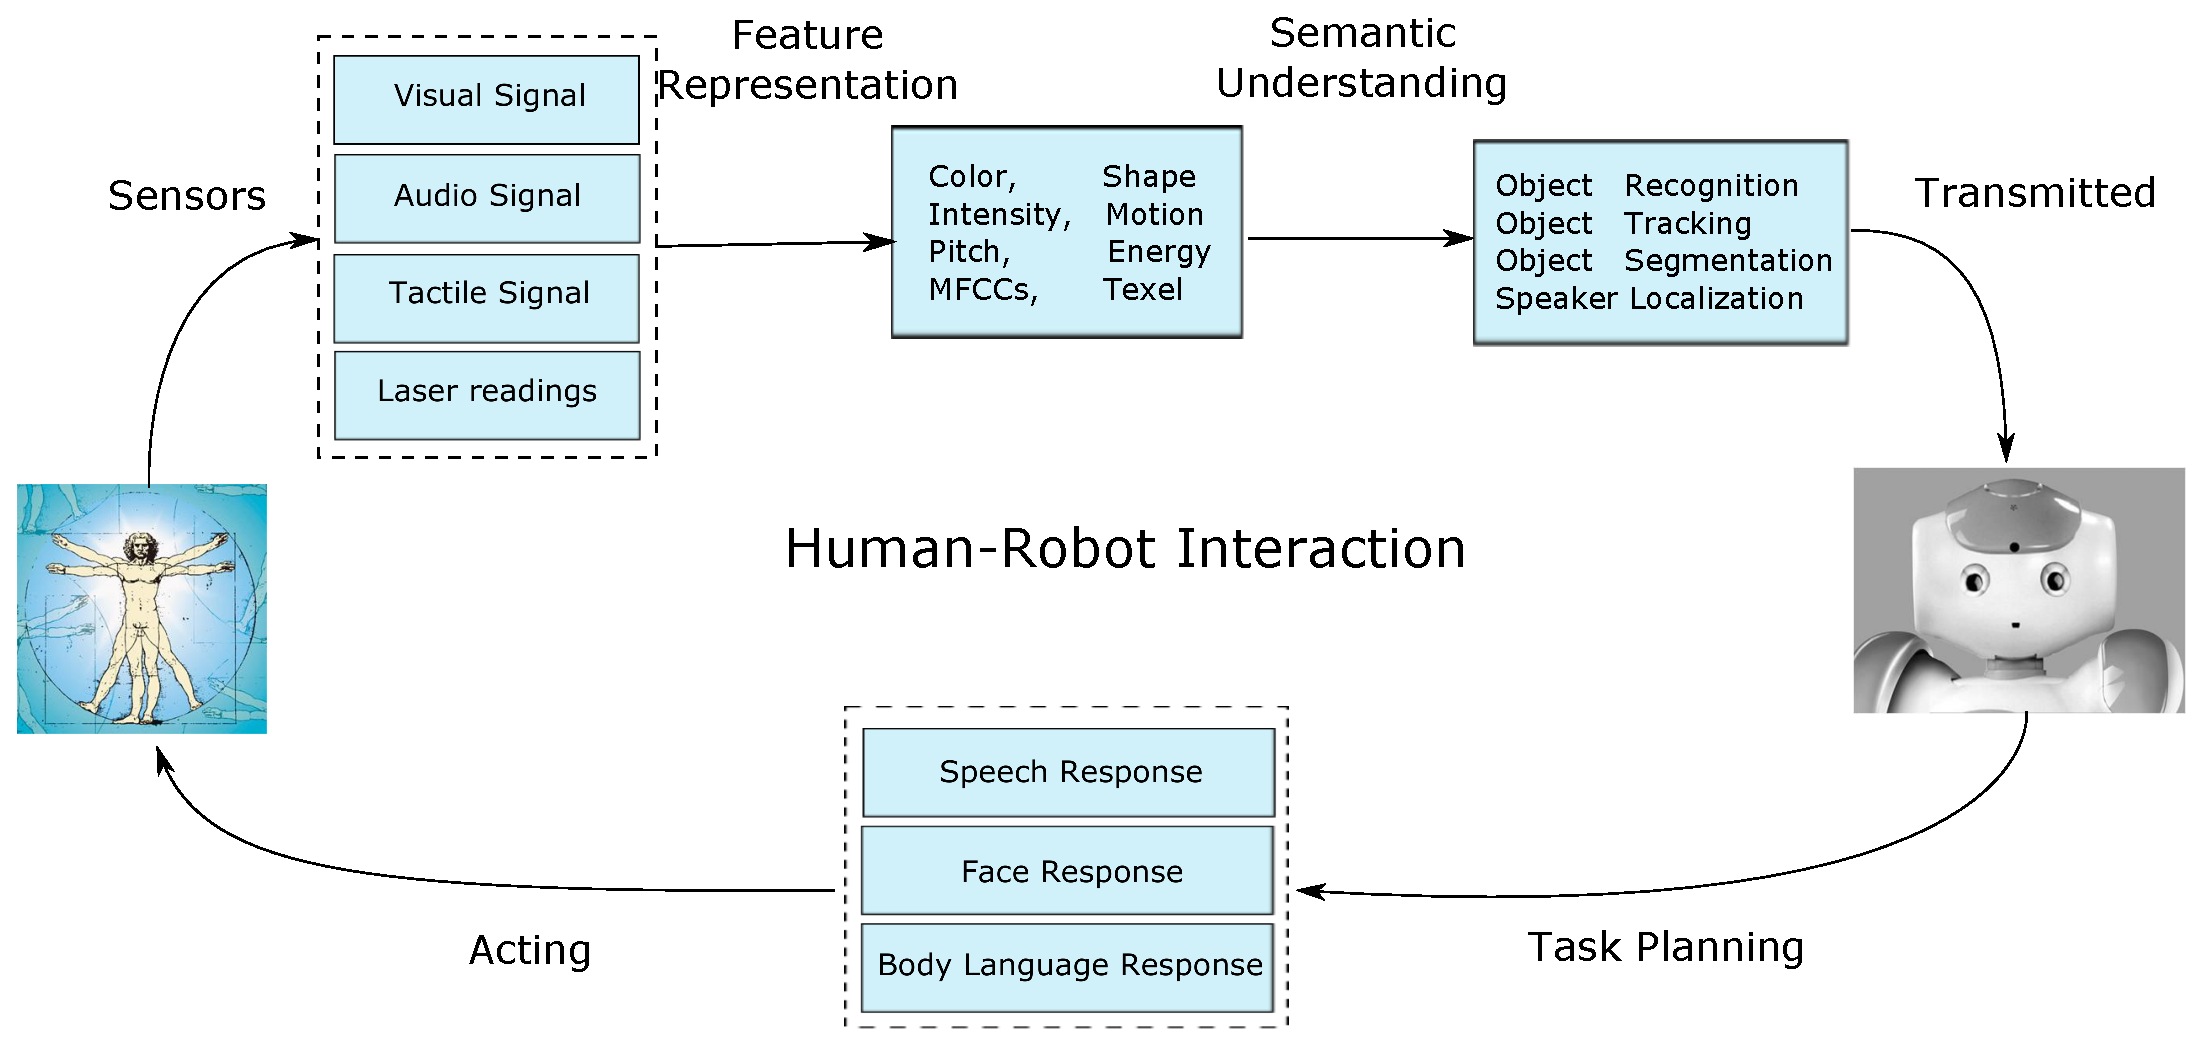
\includegraphics[width=1\textwidth]{assets/hri_perception.eps}
\caption[Perception in Human Robot interaction]{Perception in Human Robot interaction. {Adopted from \cite{yan2014survey}}}
\label{fig:hri_perception}
\end{figure}
	For human-robot interaction, perception is one of the most important capabilities. We can see from the Figure~\ref{fig:hri_perception} that the perception systems plays a major role in HRI as it acts as a communication channel between the social robots and the outside environment. There have been recent surveys on perception methods for human-robot Interaction in the context of social robots\cite{yan2014survey}. This study made an extensive survey on the perception system available in almost all the existing social robots. Moreover it also presented techniques used for the semantic understanding in each of the social robots considered. This study acts as a knowledge base for the HRI designers to make a choice of perception method that matches their requirements. In this section we describe the perception system requirments and possible solutions.
\subsection{Requirements}
	There are four major classes of signals captured by a social robot. They are visual, audio, tactile and range sensors based signals. These information are collected by cameras, microphones, tactile sensors and range finders\cite{yan2014survey}. Depending on the task requirements, robots are equipped with one or many of these sensors and the sensors could be proprioceptive or exteroceptive. 
Our choice of perception system should satisfy the following requirements
\begin{itemize}
\item Precise 6-D localization of Nao and Human(s) in the environment; For the 6D pose estimation we could use standalone or a combination of the following onboard sensors: Cameras, IMUs and Odometry sensors. However onboard sensors are erroneous.
\item Sensor data should facilitate the possibility of understanding human motions. For understanding complex human motions, the available on-board sensors and computing power are not enough. So we have to consider some exteroceptive sensors that satisfy this requirement. 
\item Practical for a social interaction scenario, cheap, and reliable.
\end{itemize}
\subsection{Existing Solutions}
	Human motion capture has been mainly developed to be used in medical, ergonomics, sports, robotics and other applications. Optical motion capture is one of the traditional ways of capturing the human motion (System like VICON$^{\regmark}$ have been deployed to aquire the \emph{MOCAP} data). However the main difficulty in the traditional optical motion capture system is the neccessity to equip the subject/actor with \emph{reflective markers}. The system itself is huge, expensive to setup and has to be calibrated before using. Since the markers move relative to the skin, there is possibility of noisy measurements due to skin artifacts. Another important point to be noted is that such a huge system is not suitable for practical HRI scenarios. However \emph{MOCAP} data acts as the ground truth for most of the motion capture systems which especially use machine learning techniques.
	
	Other devices which are commonly used to capture the kinematic information are \emph{Accelerometers} and \emph{Inertial Measurement Unit(IMU)}. There are studies of understanding the human motion using IMU\cite{aoki2013segmentation} in which the human motion (arm only) is captured from IMU sensor and commercially available Wii$^{\regmark}$ remote. This work extended the motion segmentation based on joint angles acquired using the motion capture system to the angular velocity data obtained from the IMU sensors. Though 80\% auto segmentation of human motion has been reported in the work, the complete understanding of the human motion requires lot of IMU sensors to be installed on the human body which will make the human motions more constrained. Again the IMU sensors cannot satisfy all the requirements we have for our perception system.
\subsection{RGB-D Sensors}
\label{ssec:rgbd_sensors}
	The RGB-D cameras provide a convincing solution which satisfy all the above requirements. Thanks to the advancements in the gaming industry, it accelerated the development of interaction systems and thus one can now get access to a wide variety of RGB-D cameras that are cheaper and easily available. RGB-D cameras\cite{ren2013change} are active sensors that provide high resolution dense color and depth information at real time frame rates. General-purpose robot perception usually relies on either traditional optical cameras or laser rangefinders, each having advantages and disadvantages. Cameras are fundamentally limited by the loss of 3-D structure in the 3-D or two-dimensional (2-D) projection and by their dependency on lighting conditions. It is possible to recover 3-D structures from images but such a process requires high-quality images, is computationally demanding. On the other hand, laser rangefinders allow much more robust sensing at long range but they are bulky and expensive and typically provide depth only at sparse scanlines. The RGB-D cameras combine the strengths of optical cameras and laser range finders enable a complete perception solution.
\begin{figure}
\centering
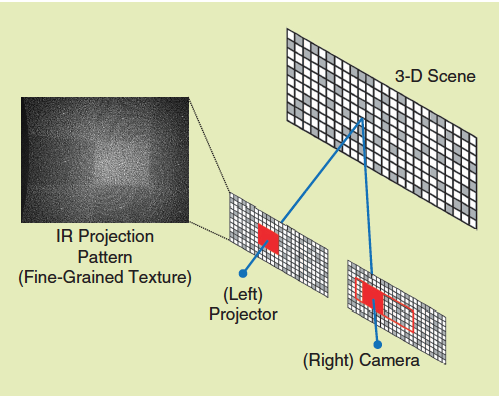
\includegraphics[width=0.5\textwidth]{assets/rgbd_activestereo.png}
\caption[Active Stereo Approach]{Active Stereo Approach. {Adopted from \cite{ren2013change}}}
\label{fig:rgbd_activestereo}
\end{figure}

	To reliably measure depth, RGB-D cameras use active sensing techniques, based on projected texture stereo, structured light, or time of flight. The technology from PrimeSense, used in the Microsoft Kinect V1\cite{Kinect2014} and Asus Xtion, depends on structured light, which projects a known IR pattern into the environment and uses the stereo principle to triangulate and compute depth. Latest Kinect V2 uses time-of-flight principle of measuring phase shift in an RF carrier.
	 
	Active stereo approaches solve the problems of depth estimation using stereo cameras by projecting a pattern, effectively painting the scene with a texture that is largely independent of the ambient lighting. Figure~\ref{fig:rgbd_activestereo} shows the basics of structured light stereo. One of the two cameras is replaced by an IR projector. The IR camera knows the locally unique projection pattern and how the pattern shifts with distance, so a local search can determine the shift (disparity) and depth can be computed through triangulation. Unlike traditional stereo rigs, RGB-D sensors do not suffer calibration problems as both the projector and IR camera exhibit low distortion. The external correspondence between the camera and the projector is determined by a factory calibration. Moreover the rigid mount ensures that the devices do not have to be recalibrated during use.
	
	 A glimpse of the readily available consumer RGB-D sensors are shown in Figure~\ref{fig:rgbd_sensors} and a study on the different available RGB-D cameras has been presented in the Table~\ref{table:rgbd_sensors}.
\begin{figure}
\centering
\begin{subfigure}[b]{0.33\textwidth}
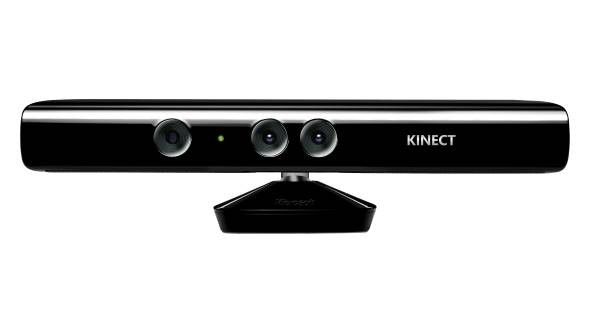
\includegraphics[width=\textwidth]{assets/kinectv1.jpg}
%http://www.microsoftstore.com/store/msusa/en_US/pdp/Kinect-for-Windows/productID.253769800
\caption{Kinect for Windows V1}
\label{fig:kinectv1}
\end{subfigure}%
\begin{subfigure}[b]{0.33\textwidth}
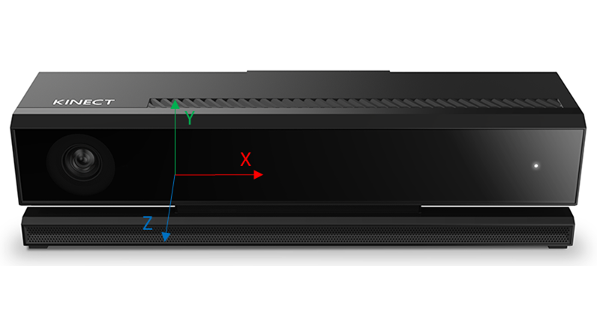
\includegraphics[width=\textwidth]{assets/kinectv2_2.png}
%http://www.microsoftstore.com/store/msusa/en_US/pdp/Kinect-for-Windows-v2-Sensor/productID.298810500
\caption{Kinect for Windows V2}
\label{fig:kinectv2}
\end{subfigure}%
\begin{subfigure}[b]{0.33\textwidth}
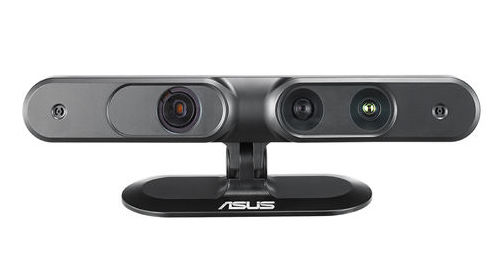
\includegraphics[width=\textwidth]{assets/asus_xtion.jpg}
%http://www.asus.com/Multimedia/Xtion_PRO_LIVE/
\caption{Asus Xtion PRO Live}
\label{fig:asus_xtion}
\end{subfigure}

\begin{subfigure}[b]{0.33\textwidth}
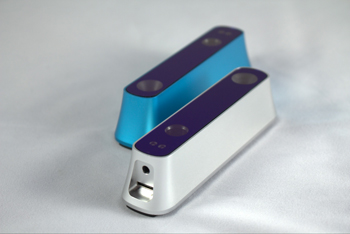
\includegraphics[width=\textwidth]{assets/structure_sensor.jpg}
%http://www.microsoftstore.com/store/msusa/en_US/pdp/Kinect-for-Windows/productID.253769800
\caption{Structure Sensor}
\label{fig:structuresensor}
\end{subfigure}%
\begin{subfigure}[b]{0.33\textwidth}
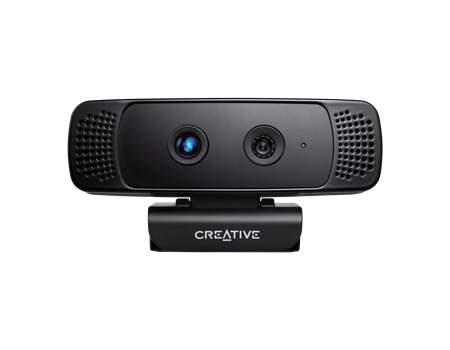
\includegraphics[width=\textwidth]{assets/creative_senz3d.png}
%http://www.microsoftstore.com/store/msusa/en_US/pdp/Kinect-for-Windows-v2-Sensor/productID.298810500
\caption{Creative Sens3D}
\label{fig:creative_senz3d}
\end{subfigure}%
\begin{subfigure}[b]{0.33\textwidth}
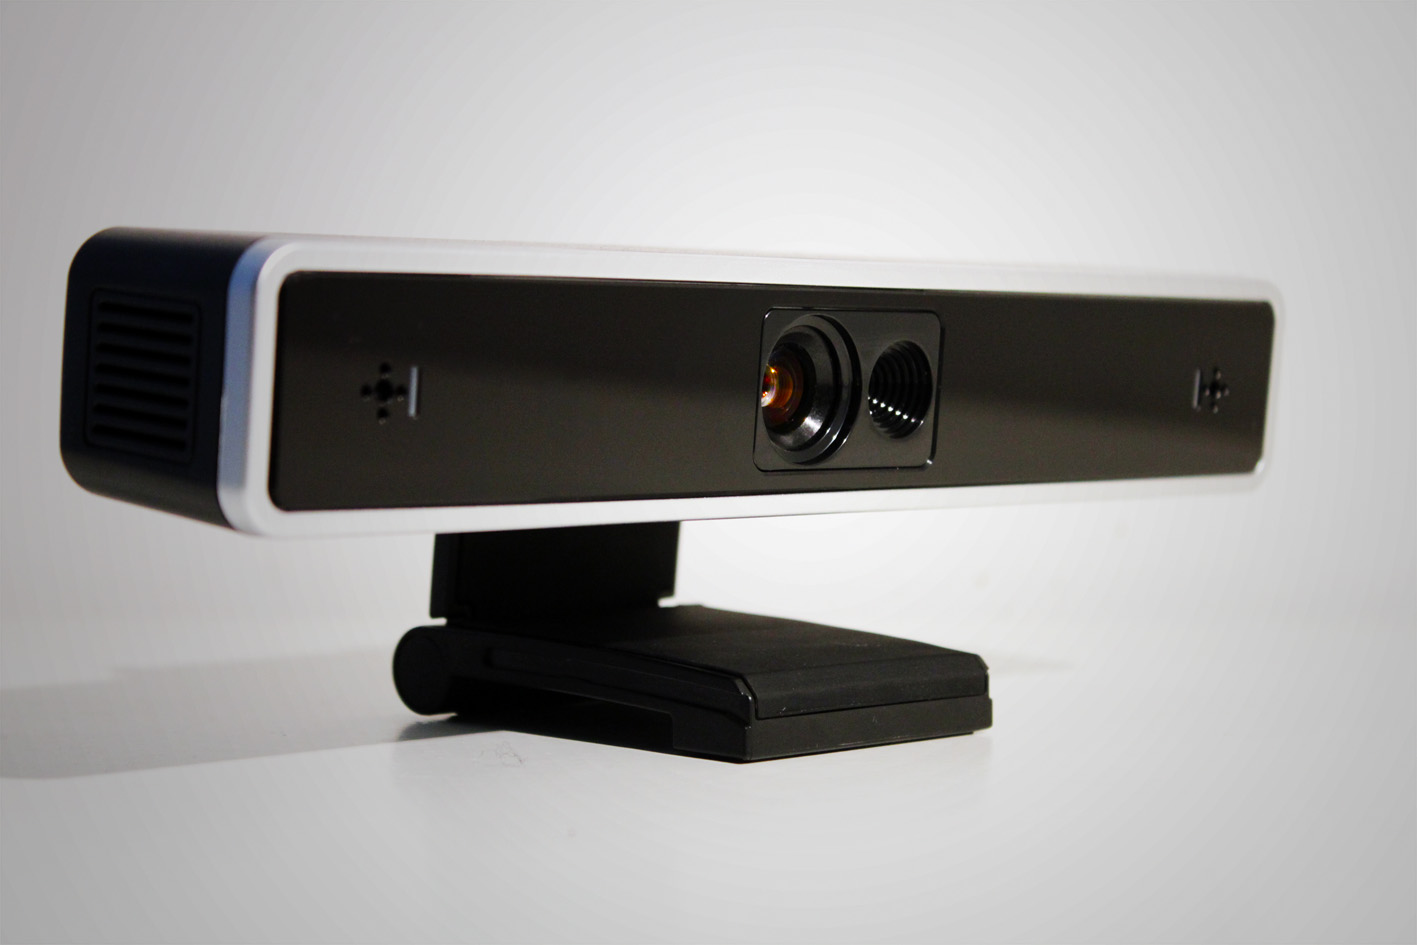
\includegraphics[width=\textwidth]{assets/depthsense_DS311.jpg}
%http://www.asus.com/Multimedia/Xtion_PRO_LIVE/
\caption{Depthsense DS$^{\regmark}$325}
\label{fig:depthsense}
\end{subfigure}
\caption[Consumer RGB-D sensors]{Consumer RGB-D sensors. {Adopted from manufacturer's site}}
\label{fig:rgbd_sensors}
%http://pressreleases.triplepointpr.com/2012/01/09/softkinetic-debuts-ultra-short-range-drivers-for-gesture-recognition-cameras-at-ces/
\end{figure}
	Among the available sensors shown in Table~\ref{table:rgbd_sensors}, Kinect V2\cite{Kinect2014} sensor has promising specifications and price. The Kinect comes with a powerful SDK\cite{KinectSDK2014} capable of performing skeleton tracking of upto 6 people (25 joints each) simultaneously out of the box. It also comes with the face detection, expression detection, gesture recognition and thumb tracking. The Kinect studio software can record the sensor data, play back and it is also possible to build gestures and train the sensor to detect when it sees them later using the Gesture builder. Though the Kinect V2 sensor works well with the Microsoft ecosystem, cross platform support is still a concern and open-source efforts in porting Kinect V2 can be found in
\begin{itemize}
\item Kinect One (Kinect v2) in ROS: \url{https://github.com/code-iai/iai_kinect2}
\item OpenNI tracker : \url{http://wiki.ros.org/openni_tracker}
\item OpenNI2 : \url{https://github.com/occipital/openni2}
\end{itemize}

\clearpage
\begin{landscape}
\Centering
\small
\begin{table}
\scriptsize
\caption{Comparative analysis on RGB-D sensors}
\label{table:rgbd_sensors}
\begin{tabularx}{600pt}{c*6{X}}
\toprule
  \textbf{Specification} & \textbf{KinectV1\footnotemark[1]} 
                         & \textbf{KinectV2\footnotemark[1]} 
                         & \textbf{Asus-Xtion Pro\footnotemark[2]} 
                         & \textbf{Structure Sensor\footnotemark[3]}
                         & \textbf{Creative Sens3D\footnotemark[4]} 
                         &  \textbf{DepthSense$^{\regmark}$325\footnotemark[5]} 
  \tabularnewline \midrule
  \multicolumn{1}{l}{Field of View}       & Vertical $43^{\circ}$; Horizontal $57^{\circ}$  
                                          & Vertical $60^{\circ}$; Horizontal $70^{\circ}$ 
                                          & Vertical $45^{\circ}$; Horizontal $58^{\circ}$; Diagonal $70^{\circ}$
                                          & Vertical $45^{\circ}$; Horizontal $58^{\circ}$ 
                                          & $74^{\circ}$
                                          & Vertical $58^{\circ}$; Horizontal $74^{\circ}$; Diagonal $87^{\circ}$
                                          \tabularnewline\midrule
                                          
  \multicolumn{1}{l}{Tilt Motor}          & Yes
  										 & No (Manual)
  										 & No 
  										 & No 
  										 & No
  										 & No 
  										 \tabularnewline\midrule
  \multicolumn{1}{l}{Skeleton Joints}     & 20, 2 skeloton
  										 & 25, 6 skeleton
  										 & - 
  										 & - 
  										 & - 
  										 & - 
  										 \tabularnewline\midrule			
  		 
  \multicolumn{1}{l}{Range (m)}           & Min: 0.4; Max $\approx$ 4.5 
  										 & Min: 0.5; Max $\approx$ 4.5
  										 & Min: 0.8; Max: 3.5
  										 & Min: 0.4; Max: 3.5  
  										 & Min: 0.5 cm; Max: 3.25 m 
  										 & Min: 0.15 $\sim$ 1; Max: 1.5 $\sim$ 4.0 
  										 \tabularnewline\midrule
  										 										 

  \multicolumn{1}{l}{Frame rate }         & RGB: 640x480, 30 FPS, 4:3; Depth: 320x420
  										 & RGB: 1920x1080, 30 FPS, 16:9; Depth: 512x424
  										 & RGB: 1280x1024, Depth: 640x480 (30 fps), 320x240 (60 fps)
  										 & RGB: 640x480 (30 fps), 320x240 (60 fps)
  										 & RGB: 1280x720 (30 fps), Depth: 320x240 (30 fps)
  										 & RGB: 1280x720 (30 fps), Depth: 320x240 (30 fps)
  										 \tabularnewline\midrule
  										 
  \multicolumn{1}{l}{Interface}           & USB 2.0
  										 & USB 3.0
  										 & USB 2.0/3.0 
  										 & USB 2.0
  										 & USB 2.0
  										 & USB 2.0
  										 \tabularnewline\midrule	
  
  \multicolumn{1}{l}{OS}                 & Win 7, Win 8
  										 & Win 8
  										 & Win XP,Vista,7,8; Ubuntu, Android
  										 & iOS, Android, Win
  										 & Win 32/64: XP,Vista,7,8;
  										 & Win 32/64: 7,8; 
  										 \tabularnewline\midrule	
  										 										 								
  
  \multicolumn{1}{l}{SDK}                & Kinect for Windows V1.x SDK(C++/C\#)
  										 & Kinect for Windows V2 SDK(C++/C\#)
  										 & OpenNI SDK (C++ / C\# /JAVA)
  										 & Structure Framework(iOS), OpenNI(C++)
  										 & Intel perceptual computing (PC) SDK 
  										 & The Interface is You (iisu) Framework, Intel PC SDK (C++/C\#)
  										 \tabularnewline\midrule	
  										 
 \multicolumn{1}{l}{Audio Input}        &  Microphone array-4, 16 KHz, Mono PCM, 24 bit ADC, Echo cancellation        											and noise suppression 
  										&  Microphone array-4, 48 KHz, Mono PCM, 24 bit ADC, Echo cancellation        											and noise suppression 
  										&  2 - Microphones 
  										&  - 
  										&  Dual array microphone 
  										& 2 built-in microphone
  										\tabularnewline
  										\bottomrule
\end{tabularx}
\end{table}
\footnotetext[1]{\url{http://www.microsoft.com/en-us/kinectforwindows/}}
\footnotetext[2]{\url{http://www.asus.com/Multimedia/Xtion_PRO_LIVE/specifications/}}
\footnotetext[3]{\url{http://structure.io/developers}}
\footnotetext[4]{\url{http://fr.creative.com/p/web-cameras/creative-senz3d}}
\footnotetext[5]{\url{http://www.softkinetic.com/Store/ProductID/6}}
\end{landscape}

\section{Summary}